\documentclass[]{BasiliskReportMemo}
\usepackage{AVS}

\newcommand{\submiterInstitute}{Autonomous Vehicle Simulation (AVS) Laboratory,\\ University of Colorado}

\newcommand{\ModuleName}{thrMomentumManagement}
\newcommand{\subject}{Reaction Wheel Angular Momentum Dumping Management Module}
\newcommand{\status}{Initial Document draft}
\newcommand{\preparer}{H. Schaub}
\newcommand{\summary}{This module reads in the Reaction Wheel (RW) speeds, determines the net RW momentum, and then determines the amount of angular momentum that must be dumped.  A separate thruster firing logic module called {\tt thrMomentumDumping} will later on compute the thruster on cycling.      }


\begin{document}


\makeCover


%
%	enter the revision documentation here
%	to add more lines, copy the table entry and the \hline, and paste after the current entry.
%
\pagestyle{empty}
{\renewcommand{\arraystretch}{1.1}
\noindent
\begin{longtable}{|p{0.5in}|p{4.5in}|p{1.14in}|}
\hline
{\bfseries Rev}: & {\bfseries Change Description} & {\bfseries By} \\
\hline
Draft & Initial document creation & H. Schaub \\
0.1 & Updated the sign of $\leftexp{B}{\Delta\bm H}$ & H. Schaub \\
1.0 & Updated document for code review & H. Schaub \\
1.1 & Updated module assumption section & R. Calaon \\
\hline

\end{longtable}
}

\newpage
\setcounter{page}{1}
\pagestyle{fancy}

\tableofcontents
~\\ \hrule ~\\

\begin{figure}[htb]
	\centerline{
	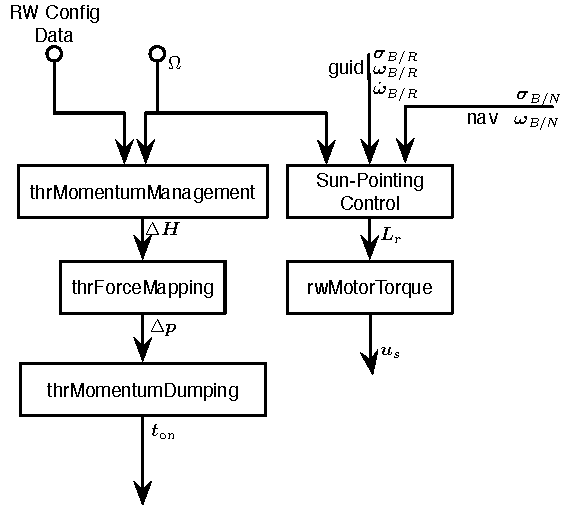
\includegraphics[]{Figures/rwMomentumOverview}
	}
	\caption{Overview of the Modules Used to Perform Reaction Wheel Angular Momentum Dumping.}
	\label{fig:Fig1}
\end{figure}

\section{Module Description}
\subsection{Overall RW Momentum Management Outline}
To manage the Reaction Wheel (RW) angular momentum build-up over time, a thruster-based momentum dumping strategy is used.  Figure~\ref{fig:Fig1} illustrates how the momentum dumping will occur simultaneously with an inertial pointing control solution.   The output of {\tt thrMomentumManagement} module is a $\Delta \bm H$ vector.  This output is then mapped into a thruster impulse request using the {\tt thrForceMapping} module.  Note that this latter module is designed to map a control torque vector into thruster forces.  If the input torque and output force sets are multiplied by time,  the same module also functions to map a desired angular momentum changes vector $\Delta H$ into a set of thruster impulse requests.  The final module {\tt thrMomentumDumping} in the series takes the thruster impulse requests and determines a thruster firing sequence to achieve this desired momentum change.  The spacecraft attitude is held constant by simultaneously having a RW control module holding an inertial attitude.  The process of holding the desired attitude leads to the RWs despinning to the desired level due the external thruster disturbances.  


\subsection{Momentum Management Algorithm}
Assume the spacecraft contains $N_{\text{RW}}$ RWs. The net RW angular momentum is given by
\begin{equation}
	\bm h_{s} = \sum_{i=1}^{N_{\text{RW}}} \hat{\bm g}_{s_{i}} J_{s_{i}} \Omega_{i}
\end{equation} 
where $\hat{\bm g}_{s_{i}}$ is the RW spin axis, $J_{s_{i}}$ is the spin axis RW inertia and $\Omega_{i}$ is the RW speed rate about this axis.  
Because the inertial attitude of the spacecraft is assumed to be held nominally steady the body-relative RW cluster angular momentum rate can be approximated as 
\begin{equation}
	\dot{\bm h}_{s} = \frac{\leftexp{B}{\D}\bm h_{s}}{\D t} + \bm\omega_{B/N} \times \bm h_{s} \approx \frac{\leftexp{B}{\D}\bm h_{s}}{\D t}
\end{equation}






\begin{figure}[tp]
	\centerline{
	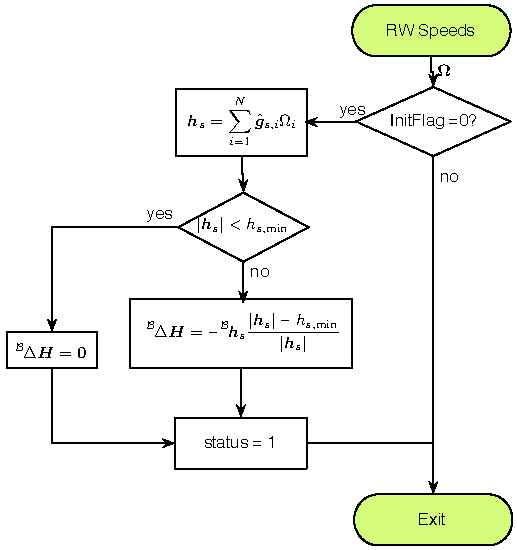
\includegraphics[]{Figures/rwMomentumManagement}
	}
	\caption{Overview of the Reaction Wheel Angular Momentum Management Module.}
	\label{fig:Fig2}
\end{figure}

Figure~\ref{fig:Fig2} illustrates the logic of the RW angular momentum dumping management module.  Let $h_{s,\text{min}}$ be lower bound that the RW momentum dumping strategy should achieve.  The desired net change in inertial angular momentum is thus determined through
\begin{equation}
	\leftexp{B}{\Delta}\bm H = -\leftexp{B}{\bm h}_{s} \frac{
		|\bm h_{s}| - h_{s,\text{min}}
	}{|\bm h_{s}|} 
\end{equation}

This strategy requires a thruster firing solution which creates this desired $\leftexp{B}{\Delta}\bm H$ over the duration of the momentum dumping.  The goal of the RW momentum management module is to simply compute if a $\leftexp{B}{\Delta}\bm H$ is required, or set it equal to zero if the RW momentum is too small.  Not that this module will only compute $\leftexp{B}{\Delta}\bm H$ once.  Either it is zero or non-zero.  To reuse this momentum management module, the reset() function must be called.


\begin{figure}[h]
	\centerline{
		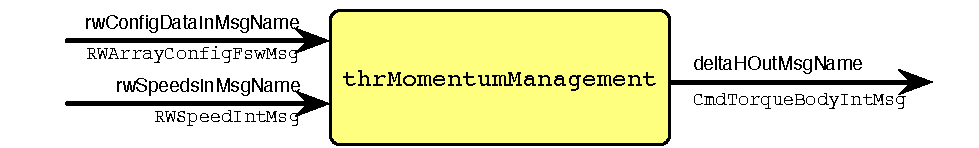
\includegraphics{Figures/moduleImg}
	}
	\caption{Illustration of the module input and output messages.}
	\label{fig:moduleImg}
\end{figure}





\subsection{Module Messages}
The module input and output messages are illustrated in Figure~\ref{fig:moduleImg}.  The module has a single output message of type {\tt CmdTorqueBodyIntMsg} which contains the desired momentum change $\leftexp{B}{\Delta}\bm H$.  

There are 2 required input messages.  The message of type {\tt RWArrayConfigMsg} is read in during the {\tt Reset()} method and provides the RW configuration states.  The message of type {\tt RWSpeedMsg} provides the current RW speeds and is read in during the {\tt Update()} method.

\subsection{{\tt Reset()} Method}
The {\tt Reset()} method reads in the RW configuration message and then resets the flag to do the angular momentum checking.  The goal here is to do this momentum checking only once after the reset function is called, rather than doing this checking autonomously.  









\section{Module Functions}
\begin{itemize}
	\item \textbf{Perform a single angular momentum check after reset}: The module should only do this momentum check once after the {\tt Reset()} method is called.
	\item \textbf{Create an output message with the desired RWA momentum change}: The output is used by a separate module to determine a momentum dumping actuation implementation.  
\end{itemize}

\section{Module Assumptions and Limitations}
The module assumes the spacecraft is holding a steady inertial orientation during the momentum dumping maneuver. This module and the cascading two modules used to perform momentum dumping do not work when run at simulation time $t=0$. For the modules to work as intended, the user needs to call \texttt{Reset()} on this module at a simulation time $t \neq 0$, at which point the amount of momentum to be dumped is computed.








\section{Test Description and Success Criteria}
A module unit test is created which creates the required input messages and runs the module for a single iteration.  Two cases are considered where the minimum RWA momentum threshold is exceed or not.




\section{Test Parameters}
The simulation is setup with 4  RWs with identical $J_{s}$ values.  
The unit test verifies that the module output  message vector matches expected values.
\begin{table}[htbp]
	\caption{Error tolerance for each test.}
	\label{tab:errortol}
	\centering \fontsize{10}{10}\selectfont
	\begin{tabular}{ c | c } % Column formatting, 
		\hline\hline
		\textbf{Output Value Tested}  & \textbf{Tolerated Error}  \\ 
		\hline
		{\tt torqueRequestBody}        & 1e-05	   \\ 
		\hline\hline
	\end{tabular}
\end{table}




\section{Test Results}
All permutations of the test passed:
\begin{table}[h]
	\caption{Test results}
	\label{tab:results}
	\centering \fontsize{10}{10}\selectfont
	\begin{tabular}{c | c  } % Column formatting, 
		\hline\hline
		\textbf{hsMinCheck} 	&\textbf{Pass/Fail} \\ 
		\hline
	   0	   			& \input{AutoTeX/passFail0} \\ 
	   1 	   			& \input{AutoTeX/passFail1} \\ 
	   \hline\hline
	\end{tabular}
\end{table}












\section{User Guide}
The module configurable parameters include:
\begin{itemize}
	\item {{\tt hs\_min} Parameter}:
This parameter dictates the desired lower ceiling of the RW cluster angular momentum.  It must be set prior to calling the routine.  
\end{itemize}



\end{document}
